\chapter{Hardware Architecture}

\section{System Overview}
The hardware architecture is centred around an ESP32-S3 microcontroller, chosen for its dual-core processing capabilities, allowing task parallelisation between sensor polling and the main control loop. The sensor suite consists of four infrared (IR) sensors, a Time-of-Flight (ToF) distance sensor, and an MPU-6050 Inertial Measurement Unit (IMU). A dual H-bridge motor driver translates the control signals into physical movement.

\begin{figure}[h]
    \centering
    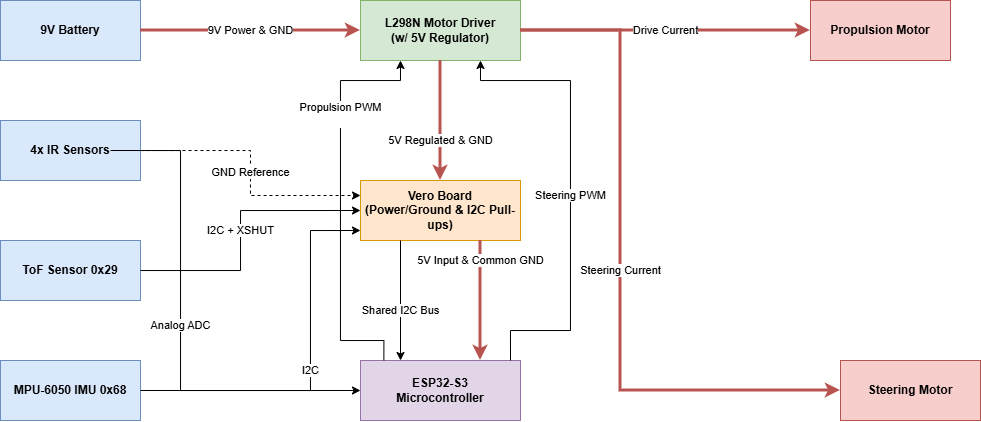
\includegraphics[width=1.2\textwidth]{images/HardwareArchitecture.drawio.png}
    \caption{Overall hardware architecture showing the ESP32-S3, sensor suite, and motor driver interfaces}
    \label{fig:hardware_architecture}
\end{figure}

\section{Component Mounting \& Integration}
Custom 3D-printed mounts were designed to secure the electronics and sensor suite to the chassis robustly. The ESP32-S3 microcontroller and the 9V power supply battery are housed in dedicated mounts positioned near the rear of the vehicle. 

The ToF sensor is mounted securely at the front of the vehicle to detect forward obstacles. The four IR sensors are positioned at each corner (front-left, front-right, rear-left, and rear-right) using custom 3D-printed mounts attached to the tire rims, ensuring consistent distance from the floor to detect tape boundaries accurately. Finally, the IMU is mounted underneath the motor driver, near the vehicle's centre of gravity (CoG), to provide reliable yaw feedback.

\todo[inline, color=blue!20]{Insert 3D CAD models and physical placement diagrams of the ESP, battery, ToF, and IR mounts here}

\section{Wiring and Pin Allocation}
The ESP32-S3 interfaces with the peripherals via ADC channels, I2C, and digital PWM pins. The pin allocation was carefully chosen to avoid conflicts, particularly avoiding the use of strapping pins or ADC channels that are active during boot for the motor PWM logic.

\subsection{Motor Control Pins}
The dual H-bridge motor driver requires four PWM signals to govern the forward/backward propulsion and left/right steering:
\begin{itemize}
    \item Left Steering: \texttt{GPIO12}
    \item Right Steering: \texttt{GPIO13}
    \item Front Propulsion: \texttt{GPIO14}
    \item Back Propulsion: \texttt{GPIO15}
\end{itemize}

\subsection{Infrared Sensors (ADC)}
The analog outputs from the four IR sensors are routed to the ESP32 ADC channels:
\begin{itemize}
    \item Front Right: \texttt{ADC1\_CH7}
    \item Front Left: \texttt{ADC1\_CH6}
    \item Rear Right: \texttt{ADC1\_CH5}
    \item Rear Left: \texttt{ADC1\_CH4}
\end{itemize}

\subsection{I2C Bus (ToF \& IMU)}
To conserve GPIO pins, the ToF sensor (address \texttt{0x29}) and the MPU-6050 IMU (address \texttt{0x68}) share a single I2C bus:
\begin{itemize}
    \item SCL: \texttt{GPIO2}
    \item SDA: \texttt{GPIO1}
    \item ToF XSHUT: \texttt{GPIO9}
\end{itemize}

\section{Power Distribution and Custom Vero Board}
A custom Vero board serves as a central power and communications distribution hub for the vehicle, ensuring robust and reliable electrical connections across all subsystems.

\begin{itemize}
    \item \textbf{Grounding:} The four IR sensors, ESP32, ToF, and IMU share a common ground. These are routed to the Vero board and tied to the motor driver ground to establish a consistent reference voltage across the entire system.
    \item \textbf{3.3V Power:} A dedicated distribution rail on the Vero board splits the 3.3V supply from the ESP32 to power the low-voltage sensor peripherals.
    \item \textbf{I2C Pull-ups:} The I2C communication lines (SCL and SDA) rely on pull-up resistors to maintain a logic high during idle states. These resistors are integrated directly into the Vero board circuit.
\end{itemize}

\begin{figure}[h]
    \centering
    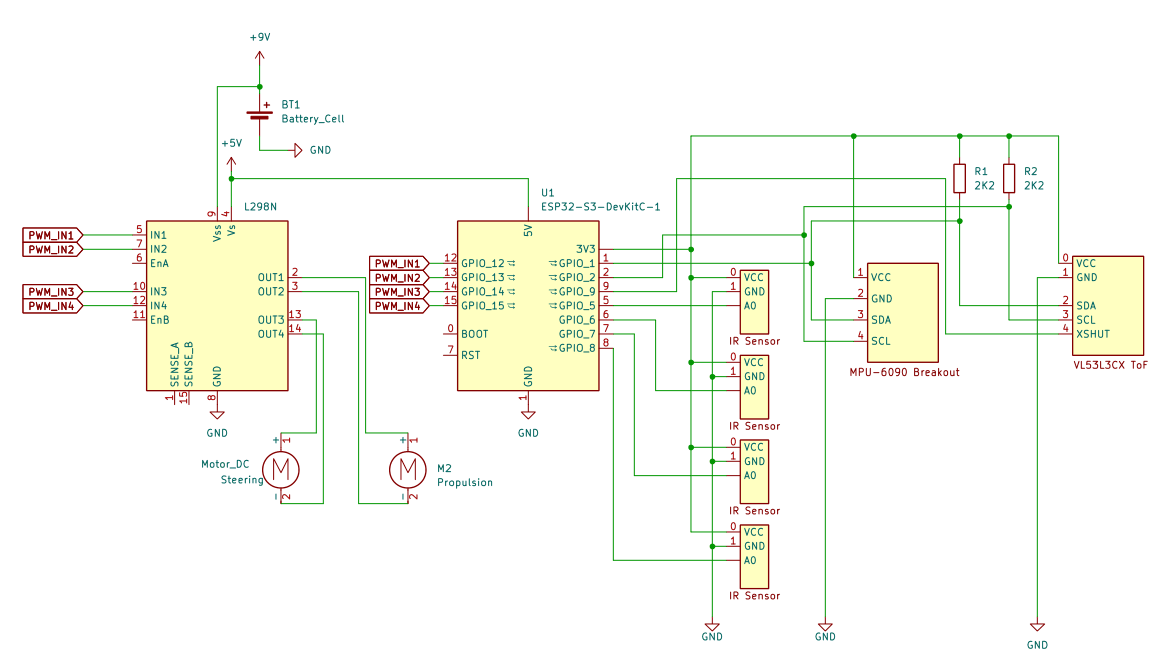
\includegraphics[width=1.2\textwidth]{images/schematic-1.png}
    \caption{Electrical schematic of the final hardware wiring and signal distribution}
    \label{fig:hardware_schematic}
\end{figure}
